% This is the magic command for latextools(ST3)
%! TEX program = latexmk -xelatex
\XeTeXgenerateactualtext=1

%%%%%%%%%%%%%% 文字コードについて %%%%%%%%%%%%%%
% Windows では標準で文字コードが Shift-JIS に  %
% である事が多いが、TeX のソースコードは UTF-8 %
% 書くことを推奨する                           %
%%%%%%%%%%%%%%%%%%%%%%%%%%%%%%%%%%%%%%%%%%%%%%%%

% 行頭に '%' をつけるとコメントになる

%%% ドキュメントクラスの設定 %%%
% 基本的にここは変更しない
% 文章全体の文字サイズを変えたい場合は 'XXpt' を変更すること
\documentclass[a4paper, twocolumn, xelatex, 10pt, ja=standard, Ligatures=TeX]{bxjsarticle}

%%% プレアンブル ---ここから %%%

% scaleboxを使うためのおまじない
\usepackage{graphicx}

% Preamble.tex のインポート
% This is the magic command for latextools(ST3)
%!TEX root = ./Report.tex

%%%%%%%%%%%%%%%%%%%%%%%%%%%%%%%%%%%%%%%%%%%%%%
%%%%%%%%%%%%%%%  各種設定  %%%%%%%%%%%%%%%%%%%
%%%%%%%%%%%%%%%%%%%%%%%%%%%%%%%%%%%%%%%%%%%%%%

\setpagelayout{top=20truemm, bottom=20truemm, left=12truemm, right=12truemm}

\usepackage{xeCJK}
\usepackage{graphicx}
\usepackage{xcolor, color}
\usepackage{here}
\usepackage{ascmac}
\usepackage[hyphens]{url}
\urlstyle{tt}

%%%%%%%%%%%%%%%%%%%%%%%%%%%
%%% フォント指定(XeTeX) %%%
%%%%%%%%%%%%%%%%%%%%%%%%%%%

%% 1. macOS ユーザー向け設定
%% Hiragino, Helvetica, TimesNewRoman, RictyDiminishedDiscord  
	% \usepackage{fontspec}
	% % serifフォント(日本語)
	% \setCJKmainfont[BoldFont={HiraginoSans-W6}]{HiraMinProN-W3}
	% % sans-serifフォント(日本語)
	% \setCJKsansfont[BoldFont={HiraginoSans-W6}]{HiraginoSans-W3}
	% % serifフォント(欧文)
	% \setmainfont[ItalicFont={HelveticaNeue-LightItalic}, BoldFont={HelveticaNeue-Medium}, BoldItalicFont={HelveticaNeue-MediumItalic}]{TimesNewRomanPSMT}
	% % sans-serifフォント(欧文)
	% \setsansfont[ItalicFont={HelveticaNeue-LightItalic}, BoldFont={HelveticaNeue-Medium}, BoldItalicFont={HelveticaNeue-MediumItalic}]{HelveticaNeue-Light}

	% \setmonofont[ItalicFont={RictyDiminishedDiscord-Oblique}, BoldFont={RictyDiminishedDiscord-Bold}, BoldItalicFont={RictyDiminishedDiscord-BoldOblique}]{RictyDiminishedDiscord-Regular}
	% \setCJKmonofont[ItalicFont={RictyDiminishedDiscord-Oblique}, BoldFont={RictyDiminishedDiscord-Bold}, BoldItalicFont={RictyDiminishedDiscord-BoldOblique}]{RictyDiminishedDiscord-Regular}

% 2. NotoSansCJKjp、NotoSerifCJKjp、NotoSans、NotoSerif、RictyDiminishedDiscord
	\usepackage{fontspec}
	% serifフォント(日本語)
	\setCJKmainfont[BoldFont={NotoSansCJKjp-Medium}]{NotoSerifCJKjp-Light}
	% sans-serifフォント(日本語)
	\setCJKsansfont[BoldFont={NotoSansCJKjp-Medium}]{NotoSansCJKjp-Light}
	% serifフォント(欧文)
	\setmainfont[ItalicFont={NotoSerif-LightItalic}, BoldFont={NotoSerif-Medium}, BoldItalicFont={NotoSerif-MediumItalic}]{NotoSerif-Light}
	% sans-serifフォント(欧文)
	\setsansfont[ItalicFont={NotoSans-LightItalic}, BoldFont={NotoSans-Medium}, BoldItalicFont={NotoSans-MediumItalic}]{NotoSans-Light}

	\setmonofont[ItalicFont={RictyDiminishedDiscord-Oblique}, BoldFont={RictyDiminishedDiscord-Bold}, BoldItalicFont={RictyDiminishedDiscord-BoldOblique}]{RictyDiminishedDiscord-Regular}
	\setCJKmonofont[ItalicFont={RictyDiminishedDiscord-Oblique}, BoldFont={RictyDiminishedDiscord-Bold}, BoldItalicFont={RictyDiminishedDiscord-BoldOblique}]{RictyDiminishedDiscord-Regular}


% 日付フォーマット変更
\renewcommand{\today}{\the\year/\the\month/\the\day}

% \maketitle カスタマイズ
\usepackage{titling}
\pretitle{
	\vspace{-2.3cm} % タイトルを上に詰める
	\begin{center}
		\huge\sffamily % タイトル:hugeサイズ、ゴシック体
}
\posttitle{
	\end{center}
}
\preauthor{
	\vspace{\baselineskip}
	\begin{center}
		\large\sffamily % 著者名:largeサイズ、ゴシック体
}
\postauthor{
	\end{center}
}
\predate{
	\begin{center}
		\large\sffamily % 日付:largeサイズ、ゴシック体
}
\postdate{
	\end{center}
}


% セクションのスタイル変更
\usepackage{titlesec}
\titleformat*{\section}{\Large\bfseries\sffamily}
\titleformat*{\subsection}{\large\bfseries\sffamily}
\titleformat*{\subsubsection}{\normalsize\bfseries\sffamily}


% 参照マクロ
\newcommand{\fref}[1]{\textbf{図\ref{#1}}}
\newcommand{\Fref}[1]{\textbf{式\ref{#1}}}
\newcommand{\tref}[1]{\textbf{表\ref{#1}}}


% listings 設定
% listings: ソースコードを表示するためのプラグイン
\usepackage{listings}

% コード部分の色スタイルの設定
\definecolor{bkg}{gray}{0.95}
\definecolor{def}{gray}{0.00}
\definecolor{com}{gray}{0.60}
\definecolor{key}{rgb}{0.00, 0.00, 0.75}
\definecolor{str}{rgb}{0.20, 0.50, 0.15}

% ソースコードを表示するときのキャプション名
\renewcommand{\lstlistingname}{コード}

% 書式設定
\lstset{
   % プログラミング言語
   language={C},
   % 背景色
   backgroundcolor={\color{bkg}},
   % 基本の文字スタイル
   basicstyle={\small\ttfamily\color{def}},
   % 変数の文字スタイル
   identifierstyle={\small\ttfamily\color{def}},
   % コメントの文字スタイル
   commentstyle={\color{com}},
   % 予約語の文字スタイル
   keywordstyle={\bfseries\color{key}},
   % 非予約語の文字スタイル (よくわからない)
   ndkeywordstyle={\small\color{def}},
   % 文字列リテラルのスタイル
   stringstyle={\bfseries\color{str}},
   % 枠線の設定
   % t, r, b, l: それぞれ上、右、下、左の1本線
   % T, R, B, L: それぞれ上、右、下、左の2本線
   frame={tlRB},
   % 長い文を改行するかどうか
   breaklines=true,
   % 横幅間隔の調整
   columns=[l]{fullflexible},
   % 左右のマージン
	 xrightmargin=0\zw,
   xleftmargin=1\zw,
   framexleftmargin=3pt,
   % 行番号の位置
   numbers=left,
   % 行番号のスタイル
   numberstyle={\ttfamily\small},
   % 行番号とコード本文の間の空白
	 numbersep=1\zw,
   % 行番号の刻み
   stepnumber=1,
   % コメント行の継続の設定
	morecomment=[l]{//}
}
\newcommand{\cref}[1]{\textbf{\lstlistingname\ref{#1}}}


% 行間隔の変更
\renewcommand{\baselinestretch}{0.65}

%%% プレアンブル ---ここまで %%%

%%% タイトル、筆者、日付の設定 %%%
\title{\bf 地形データを用いた土砂災害による被害家屋の検知}
\author{静岡大学\ 情報学部\ 佐治研究室 \\ 7081-0024\ 川村\ 昇平}
\date{}
% 文字としての空白を入れるときは、
% '\ ' (バックスラッシュ + 半角スペース)
% を入力する


%%%%%%%%%%%%%%%%%%%%%%%%%%%%%%%%%%%%%%%%%%%%%%
%%%%%%%%%%%%%%%%  本文 部分  %%%%%%%%%%%%%%%%%
%%%%%%%%%%%%%%%%%%%%%%%%%%%%%%%%%%%%%%%%%%%%%%

% インデントは必須ではないが、可読性のために
% インデントを推奨する


\begin{document}
	
	% タイトル生成
	\maketitle

	% 文章の大きな区切りには、 \section 環境を使用する
	\section{はじめに}
		% figure 環境:図を掲載する
		% \begin{figure}[位置指定] ... \end{figure}
		% 位置指定: h(その位置)、t(ページ上部)、b(ページ下部) 、p(図表専用ページを作成)
		% 'h' 指定が思うように行かない場合、'!h' を使用する
		% '!h' でもうまくいかない場合、'H' を使用する
		% 画像ファイルは EPS(PDF) または PNG を推奨

		% \ref を使用すると、図表番号を参照できる
		% {}に指定するものは、各図表で設定した label の名前を指定する
		% なお、\ref は番号のみを表示するだけで '表' や '図' という文字
		% まで表示してくれない。毎回 '表' や '図' を打つのはめんどくさい
		% ので、勝手に挿入してくれるマクロを作成しているので、ぜひ
		% 使っていただきたい
		% \fref : 図(Figure)の参照。「図XX」のように表示してくれる
		% \tref : 表(Table)の参照。「表XX」のように表示してくれる
		% \Fref : 式(Formula)の参照。「式XX」のように表示してくれる
		% \cref : コード(Code)の参照。「コードXX」のように表示してくれる

			% 考察でソースコードを掲載して言及したいことがある場合は、
			% 以下のフォーマットでソースコードを掲載してください

			%%% lstlisting の使い方 %%%
			%% 1. .tex ファイルに直接ソースコードを記入する場合
			% \begin{lstlisting}[caption=\texttt{キャプション表示名}, label=ラベル識別子]
			%   ここにソースコードを直接記述
			% \end{lstlisting}

		日本では土砂災害が多発しており, 迅速な救助・捜索のための災害状況把握が要求されている. 
		住宅地に被害を及ぼす土砂災害では, 家屋がどこへ流されたのかを特定することが救助・捜索の観点で重要である. 
		家屋が流された場所を特定するためには, 流された家屋がもとはどこにあったのか, 何軒の家屋がどこに流されたのか, といった情報が必要となる. 

		また, 災害状況把握の手段として, 近年ではリモートセンシング技術が注目されている. 
		リモートセンシング技術による災害状況把握手段として, 航空機による動画像撮影や航空レーザ測量が挙げられる. 
		航空レーザ測量は, 標高データが取得できる点や地図との位置合わせが容易である点などから, 動画像に比べ多角的な状況把握に有効である. 

		長谷川ら\cite{bunken01}は上空映像に対し目視で建物被害を判定する手法を提案しているが, 目視での判定は時間と人手の面でコストが高い. 
		遠藤\cite{bunken02}は地震後上空画像を用い建物被害判定を支援する手法を提案しているが, 地図と上空画像の位置合わせでずれが生じてしまうという問題がある. 
		また, 中山\cite{bunken03}は災害後上空画像やDEM(数値標高モデル)を用いて土砂領域を検出する手法を提案しているが, DEMの解像度が上空画像に比べて低く, 
		十分に画像内の地形を表現できない. 

		以上を踏まえ, 本研究では, 航空レーザ測量によって得られた災害前後地形データ等を用い, 
		土砂災害によって流出等の被害を受けた家屋を自動的に検知し, 救助・捜索の判断を支援する手法を提案する. 

	\section{提案手法}
		本研究の提案手法の概要図を\fref{figure_process}に示す. 

		\subsection{全体処理}\label{All_process}
			全体処理は, 「DSM化・オルソ化」, 「被害家屋検知」, 「結果統合」からなる. 
			入力データは災害前後の3次元点群データと建物マスクであり, 出力データは土砂災害による流出等の被害を受けた家屋領域を表示したものである. 
			DSM化・オルソ化は3次元点群データをDSM(数値表層モデル)とオルソ画像(直下視補正画像)に変換する処理であり, 
			被害家屋検知は変換されたデータと建物マスクを併せて用い被害家屋候補を検知する. 
			結果統合は, 被害家屋検知で得られた結果を用い, 土砂災害による被害家屋の検知を行う. 
			
			また, 被害家屋検知は\ref{DSM_Sabun}節から\ref{Ortho_Sabun}節で後述の通り, 「DSM活用」, 「土砂被害マスク作成」, 「画像活用」からなる. 

			\begin{figure}[H] % [H]: 位置指定
				% 図表全体を中央寄せ(centering)する
				\centering
				% 図の挿入:\includegraphics[width=幅の大きさ]{画像ファイルへのパス}
				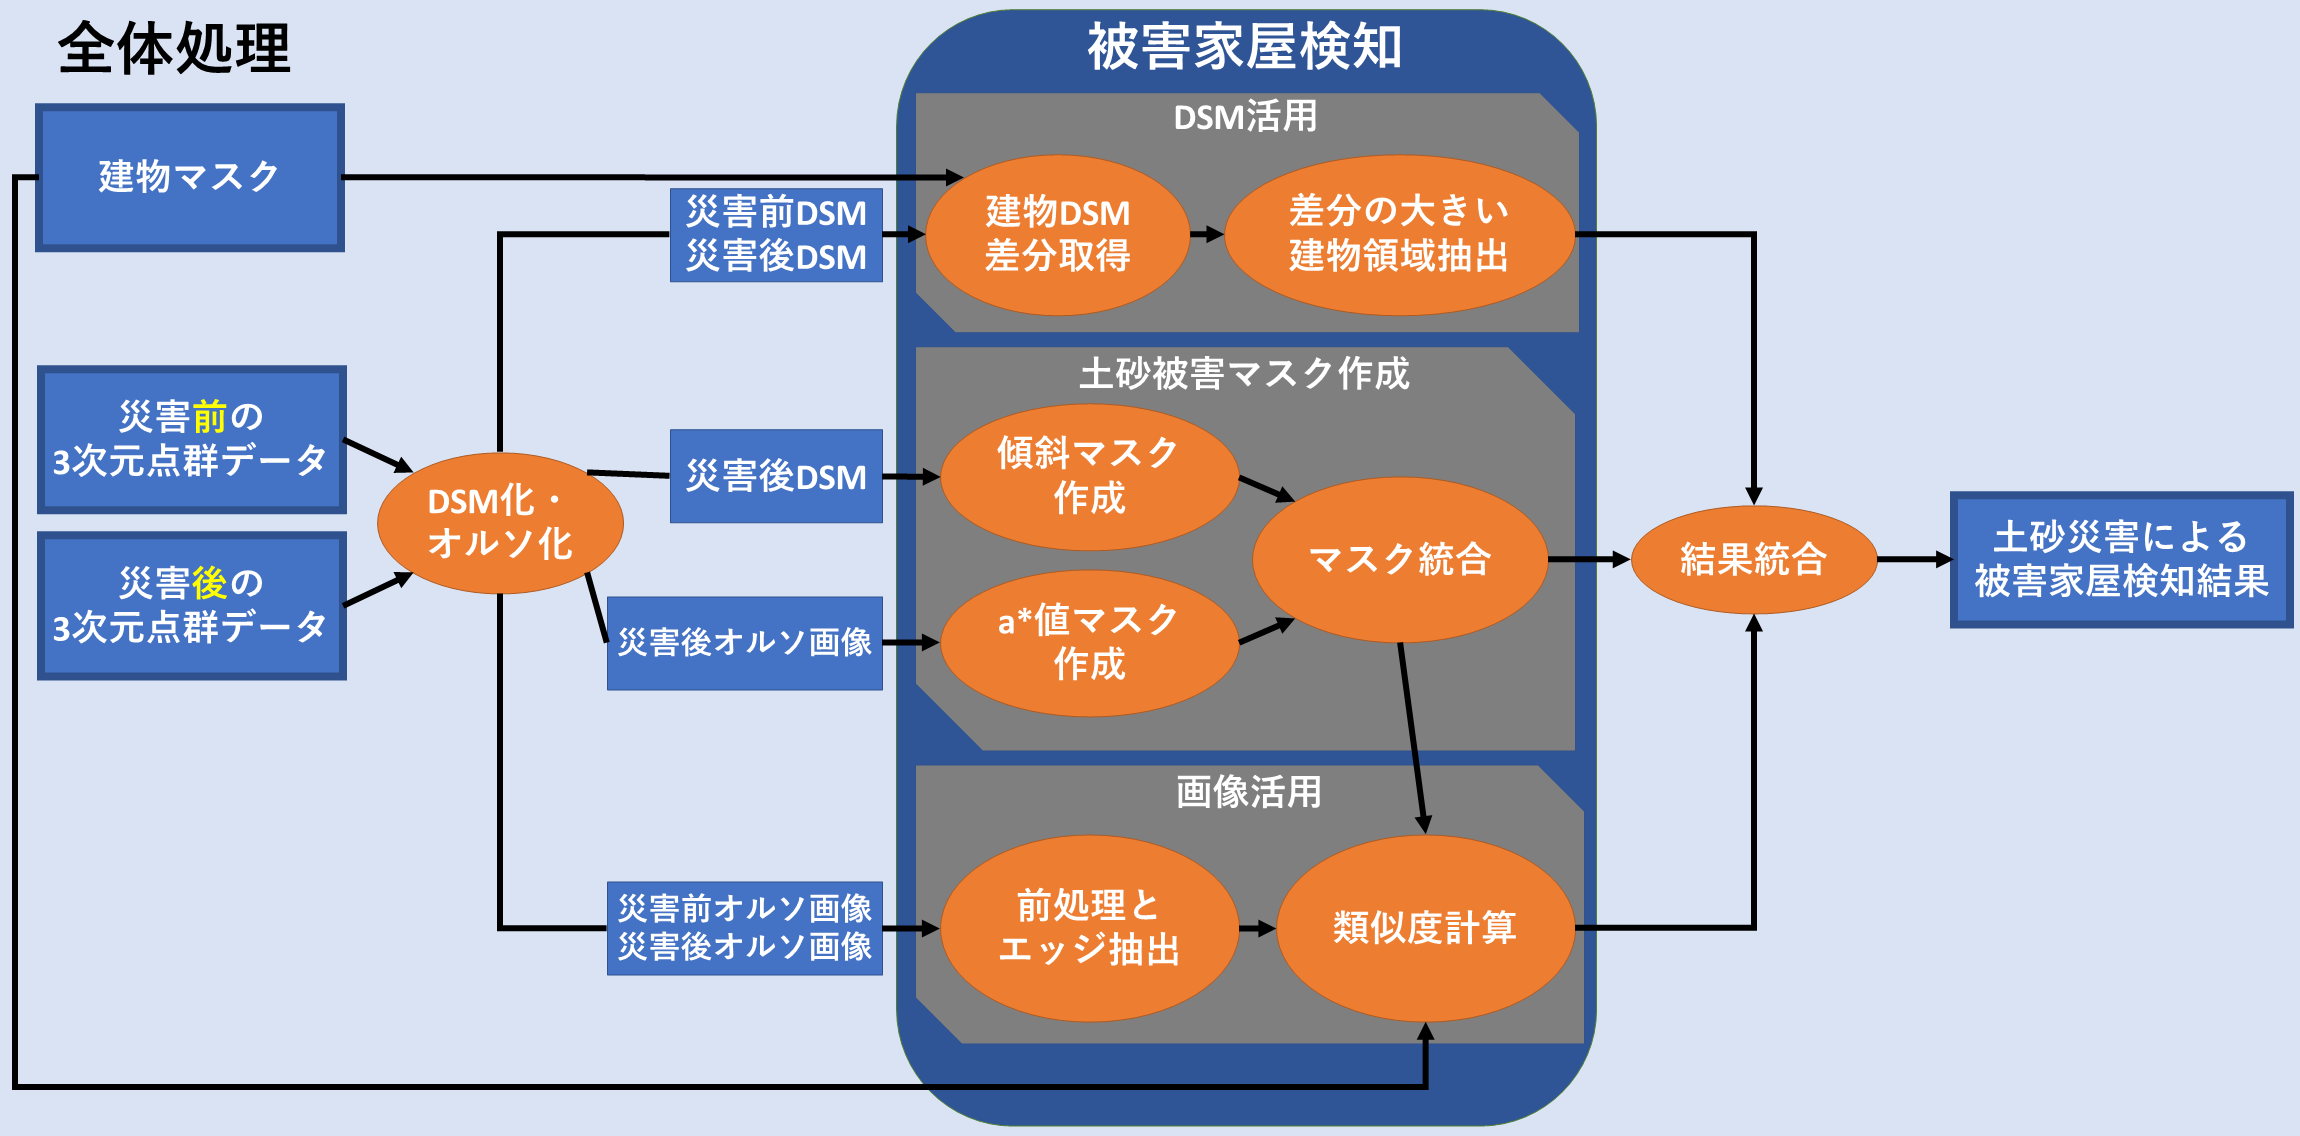
\includegraphics[width=8cm]{img/program_process/process_all.png}
				% 図のタイトル(キャプション)は下に記述する。
				\caption{提案手法の概要図}
				% ラベルの設定
				\label{figure_process}
			\end{figure}

		\subsection{DSM化・オルソ化}\label{All_process_01}
			本手法で使用する地形データは3次元点群データである. 
			3次元点群データは3次元座標・反射強度値・RGB色情報などをもつ点の集合であり, DEMやDSMのような3次元座標のみの地形データよりも幅広く活用できる. 
			DSMに変換することで標高の差分を取るのが容易になり, オルソ画像に変換することで画像としての比較が容易になる. 

			3次元点群データのDSMへの変換とオルソ画像への変換はpdal\footnote{点群データ変換のオープンソースライブラリ}\ 2.3.0を用いた. 

		\subsection{被害家屋検知【DSM活用】}\label{DSM_Sabun}
			土砂による流出等の被害を受けた家屋があった場所は, 災害前後で標高差が大きくなると考えられる. 標高差の大きい建物領域を抽出するためDSMで差分を取る.  
			
			\subsubsection{建物DSM差分取得}\label{DSM_Sabun_01}
				災害前後DSMの対応する画素同士で減算し, 建物マスクで建物領域における災害前後の標高差を取得する. 
			
			\subsubsection{差分の大きい建物領域抽出}\label{DSM_Sabun_02}
				\ref{DSM_Sabun_01}節で得られた結果で差分が閾値以上の大きさの建物領域を抽出し, 取得した領域をDSM活用による被害家屋候補とする. 

		\subsection{被害家屋検知【土砂被害マスク作成】}\label{Dosya_Mask}
			土砂被害領域を求めマスクとし, \ref{All_process_02}節での結果統合や, \ref{Ortho_Sabun_02}節で処理領域を限定するのに利用する. 
			\ref{Dosya_Mask_01}節と\ref{Dosya_Mask_02}節で二つのマスクを作り統合する. 

			\subsubsection{傾斜のマスク作成}\label{Dosya_Mask_01}
				土砂被害領域の傾斜は建物や木々の傾斜に比べて緩やかなため, 土砂被害領域を抽出するのに向いている. 
				
				最初にQGIS\footnote{オープンソースの地理情報システムソフト}\ 3.20.2を用い災害後DSMの傾斜を出し, 次にノイズの軽減を目的としてMeanShiftを用いる. 
				ここでMeanshiftは, 傾斜が類似している近傍の画素を同一の傾斜領域として統合する処理である. 最後に傾斜の小さい領域を抜き出し, 傾斜のマスクを作成する. 

			\subsubsection{a*値のマスク作成}\label{Dosya_Mask_02}
				水分を多く含んだ土砂は赤色の成分が強い茶色になるため, \ref{Dosya_Mask_01}節と同様に土砂被害領域を抽出するのに向いている. 

				最初に災害後オルソ画像を色情報の分類に適したL*a*b*表色系に変換し, 次にノイズの軽減を目的としてMeanShiftを用いる. 
				ここでMeanShiftは, L*a*b*値が類似している近傍の画素を同一のL*a*b*値領域として統合する処理である. 
				災害後オルソ画像で赤色の成分が強い領域ほど, L*a*b*表色系に変換するとa*値が大きくなる. 
				そのため最後に, 統合された領域でa*値の大きい領域を抜き出し, a*値のマスクを作成する. 

			\subsubsection{マスク統合}\label{Dosya_Mask_03}
				最初に\ref{Dosya_Mask_01}節と\ref{Dosya_Mask_02}節で得られたマスクに対し論理積をとる. 
				それだけでは不要な穴や連結成分が残るため, 次にクロージング処理とオープニング処理によってこれらを取り除く. 
				最後に残った領域の中で最も大きい領域を土砂被害領域として抽出する. その結果が土砂被害マスクである. 

		\subsection{被害家屋検知【画像活用】}\label{Ortho_Sabun}
			\ref{DSM_Sabun}節で得られる結果では, 家屋に土砂が覆い被さり標高差が生じないことによる未検知や, 
			樹木の影響およびデータ計測の誤差で標高差が生じてしまうことによる誤検知が起こり得る. 
			これらDSM活用による被害家屋候補の未検知と誤検知を減らすため, 災害前後の画像情報を比較する. 

			\subsubsection{前処理とエッジ抽出}\label{Ortho_Sabun_01}
				災害前後オルソ画像に前処理を施し, エッジを抽出することで被害家屋の検知を目指す. 

				計測時の時期や気候によって画像の色調は異なるため, オルソ画像を補正しグレースケール化する. 
				本実験に関しては災害前オルソ画像の色調が薄かったため, 災害前オルソ画像の色調を災害後オルソ画像に合わせるよう色調補正した. 
				また, 災害前オルソ画像のぼけや色調の薄さへの対策として鮮鋭化を行いエッジを強調した. 
				エッジ抽出はラプラシアンフィルタを用いたが当該フィルタではノイズを強調してしまうため, 
				エッジを保存したノイズ除去としてバイラテラルフィルタを適用してからエッジを抽出した. 

			\subsubsection{類似度計算}\label{Ortho_Sabun_02}
				\ref{Dosya_Mask}節で得られた土砂被害マスクと入力データである建物マスクの重なる領域に絞って, \ref{Ortho_Sabun_01}節で得られた災害前後のエッジのcos類似度を計算する. 
				cos類似度は, 2つの画像をベクトルとして$cos\theta$を求めそれを類似度とする. ベクトルの大きさを考慮しないためエッジの強さの差に影響を受けにくい. 
				土砂災害の被害を受けた家屋領域は類似度が低くなると考えられるため閾値以下の大きさの類似度の建物領域を抽出し, 取得した領域を画像活用による被害家屋候補とする. 

		\subsection{結果統合}\label{All_process_02}
			\ref{DSM_Sabun}節の処理結果と\ref{Ortho_Sabun}節の処理結果を統合し, 土砂災害による被害家屋の検知結果を得る. 
			このとき土砂被害を受けた家屋は土砂付近に集中すると考えられるため, \ref{Dosya_Mask}節の土砂被害マスクから一定以上離れた家屋は被害家屋から除外する. 


	\section{実験結果}
		本研究では, 2021年7月3日に静岡県熱海市伊豆山で発生した土砂災害を例に実験を行った. 
		被災地域における地形データとして, 災害前後の3次元点群データ\cite{bunken05}\cite{bunken06}と, 災害前の建物マスク\cite{bunken07}を使用する. 
		ここで用いた建物マスクとは, 基盤地図情報における「建物の外周線」を示す. 
		
		本実験で使用したデータの詳細を\tref{table_tengun}と\tref{table_mask}に示す. 
		入力する3次元点群データの一部分を例として\fref{figure_before}と\fref{figure_after}に, 
		実験1を例として建物マスクと最終的な被害家屋検知結果を\fref{figure_mask}と\fref{figure_result}に赤色で示す. 

		また, 目視により手動で作成した正解画像を用い, 家屋1軒単位の適合率・再現率・F値で精度評価した結果を\tref{table_seido}に示す.
		適合率は検知した家屋全体における正解した被害家屋の割合であり, 再現率は正解画像の被害家屋全体における検知できた被害家屋の割合であり, 
		F値は両割合の調和平均である. 

		\begin{table}[H]
			\centering
			\caption{3次元点群データ}
			\label{table_tengun}
			\small
			\begin{tabular}{ccc}
				 & 災害前 & 災害後\\
				\hline
				計測場所 & 静岡県熱海市伊豆山 & 静岡県熱海市伊豆山\\
				計測時期 & 2019年 & 2021年7月6日\\
				提供 & 静岡県 & 株式会社パスコ\\
				\hline
			\end{tabular}
		\end{table}
		\begin{table}[H]
			\centering
			\caption{建物マスク}
			\label{table_mask}
			\small
			\begin{tabular}{cc}
				\hline
				更新年月日 & 2021年1月1日\\
				提供 & 国土地理院\\
				\hline
			\end{tabular}
		\end{table}

		\begin{figure}[!h]
			\begin{minipage}{0.48\hsize}
				\centering
				\small
				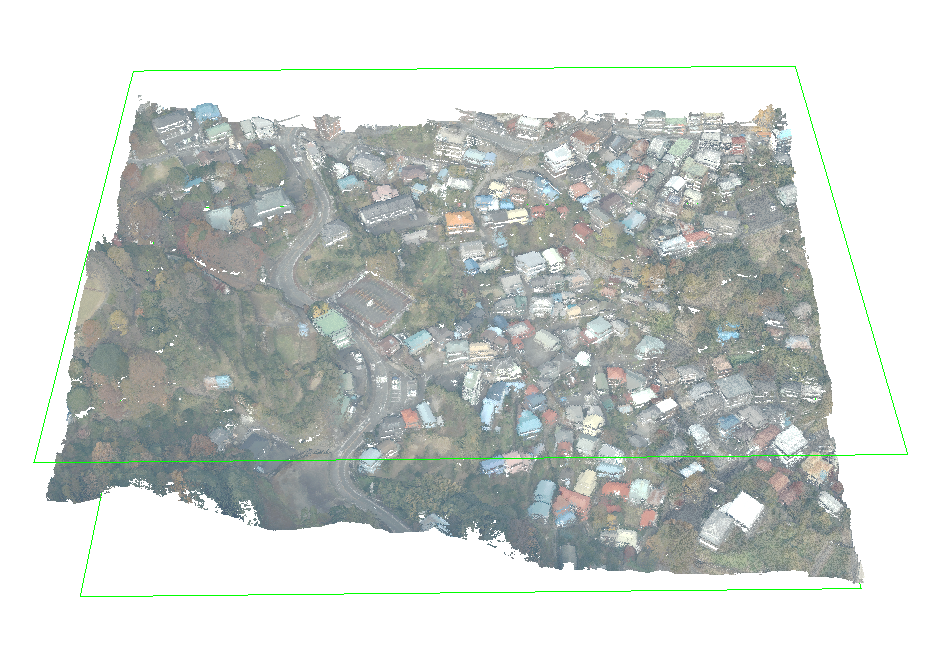
\includegraphics[width=\linewidth]{img/io_img/tengun_before.png}
				\caption{災害前の3次元点群データ}
				\label{figure_before}
			\end{minipage}
			\begin{minipage}{0.48\hsize}
				\centering
				\small
				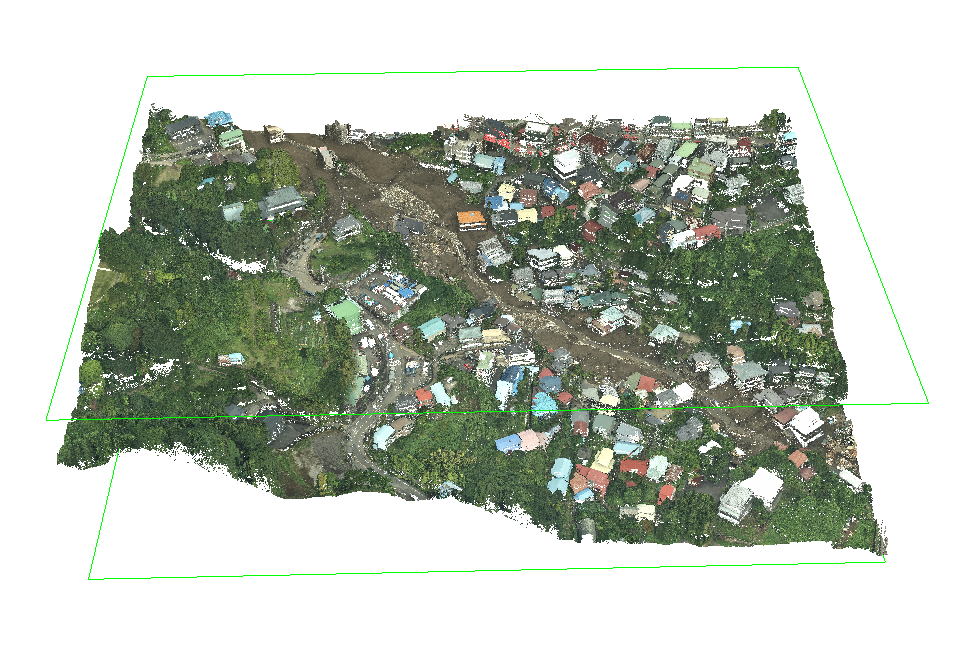
\includegraphics[width=\linewidth]{img/io_img/tengun_after.png}
				\caption{災害後の3次元点群データ}
				\label{figure_after}
			\end{minipage}
		\end{figure}

		\begin{figure}[!h]
			\begin{minipage}{0.48\hsize}
				\centering
				\small
				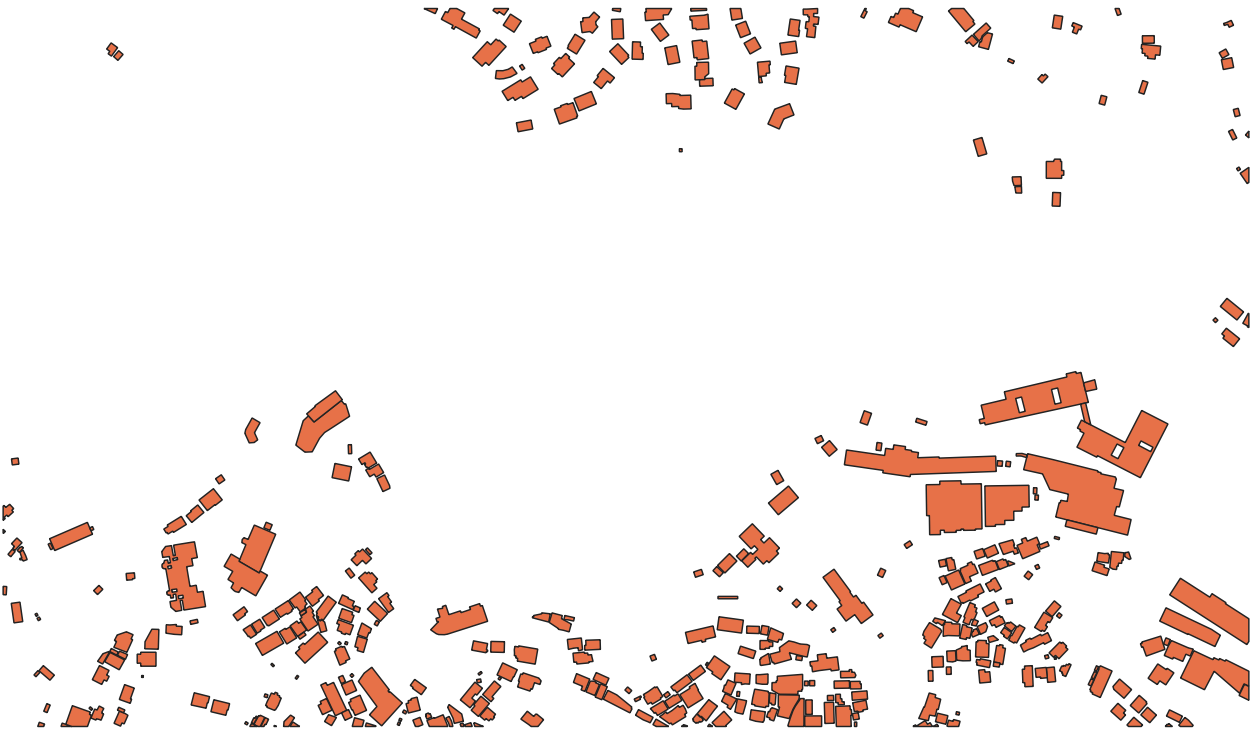
\includegraphics[width=\linewidth]{img/io_img/BLD_Mask01.png}
				\caption{建物マスク}
				\label{figure_mask}
			\end{minipage}
			\begin{minipage}{0.48\hsize}
				\centering
				\small
				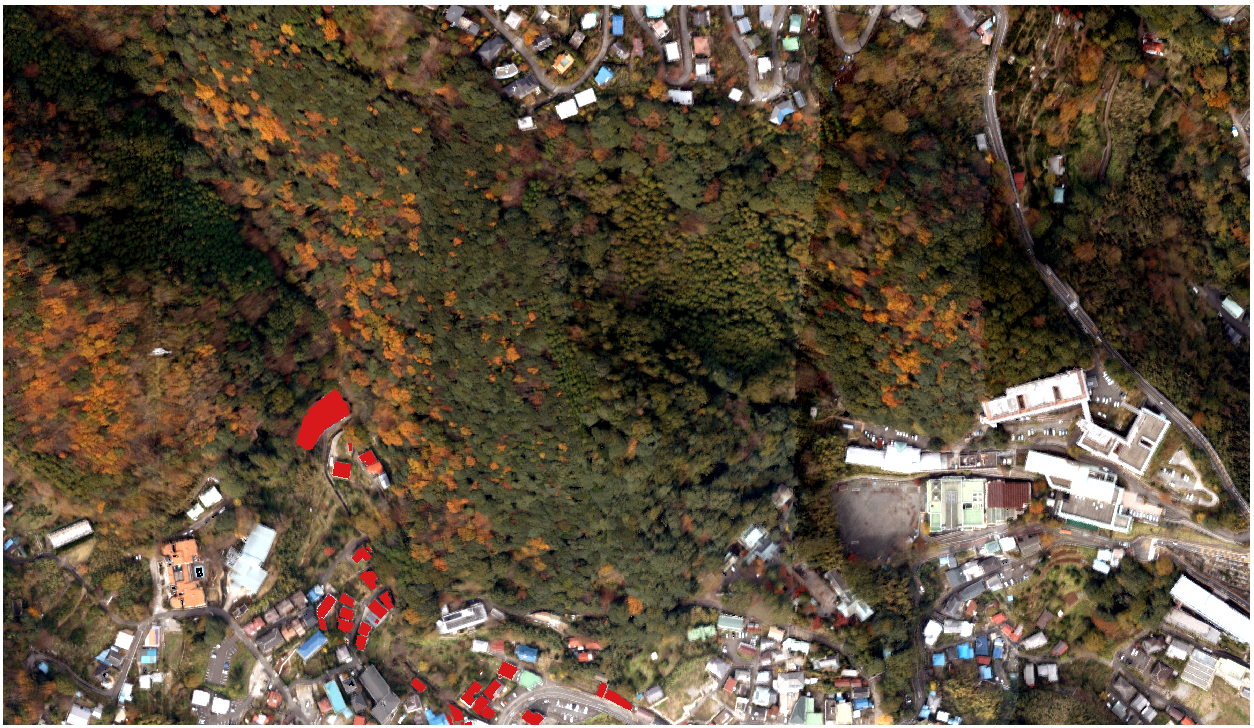
\includegraphics[width=\linewidth]{img/io_img/result01.png}
				\caption{被害家屋検知結果}
				\label{figure_result}
			\end{minipage}
		\end{figure}

		\begin{table}[H]
			\centering
			\caption{精度評価}
			\label{table_seido}
			\small
			\begin{tabular}{ccc}
				 & 実験1 & 実験2\\
				\hline
				適合率 & 0.85 & 0.84\\
				再現率 & 0.85 & 0.68\\
				F値 & 0.85 & 0.75\\
				\hline
			\end{tabular}
		\end{table}


	\section{まとめ・今後の課題}
		本研究では土砂災害前後の地形データを用いた被害家屋の検知手法を提案した. 
		高解像度のDSM・オルソ画像を取得し先行研究での問題に対処した結果, 適合率80\%以上, F値75\%以上を達成した. 

		現状の問題点としては, 土砂被害マスクの精度が原因で未検知の被害家屋が多い点や, 災害前オルソ画像のぼけが原因でエッジを適切に抽出できていない点が挙げられる. 
		前者の問題の対策としては傾斜のマスクとa*値のマスクの統合方法の改善や他のデータの利用による精度向上が考えられ, 
		後者の問題点の対策としてはエッジ抽出の前処理に画像のぼけを補正する処理の追加が考えられる. 
		
		今後は以上のような未検知の問題の解決と, 本研究をもとに, 土砂による家屋流出の全容を解明できる手法の確立を目指し, 
		災害時における救助・救援活動に貢献する予定である.  

		% \subsection{数式}
		% 	文章中に数式を入れる場合には、$x \cap y$のようにする。この場合、数式番号はつかない。
		% 	数式番号をつける場合は、このようにする。

		% 	\begin{equation}
		% 	R_{SAD}  = \sum\limits_{j = 0}^{N - 1} {\sum\limits_{i = 0}^{M - 1} {|I(i,j) - T(i,j)|} } 
		% 	\end{equation}

		% 	複数行の数式は、このように変更する。

		% 	% 複数行の数式は eqnarray 環境を用いる
		% 	% 記号を & で囲むと、その部分を各行で揃えてくれる
		% 	\begin{eqnarray}
		% 	R_{SSD} &=& \sum\limits_{j = 0}^{N - 1} {\sum\limits_{i = 0}^{M - 1} {(I(i,j) - T(i,j))^2 } }  \\
		% 	R_{SAD} &=& \sum\limits_{j = 0}^{N - 1} {\sum\limits_{i = 0}^{M - 1} {|I(i,j) - T(i,j)|} }
		% 	\end{eqnarray}

	% % \section* とすることで、番号なしのセクションを作成できる
	% \section*{謝辞} 
	% 	誰かに助言などをもらった場合は、ここに記述する。
	% 	論文などでは以下の文言が記述される事がある。
		
	% 	「本研究の一部は、〜〜技術協会からの研究助成によるものである。」

% 参考文献の表示
\bibliographystyle{junsrt}   % 参考文献の並び順を指定
\bibliography{bib/bunken.bib} % \bibliography{参考文献ファイルへのパス}

\end{document}
